\documentclass[a4paper,10pt,fleqn]{article}

\usepackage{layout}

\title{Dokumentation rc-gen}
\author{Daniel Winz}

\begin{document}
\maketitle
\clearpage
\tableofcontents
\clearpage

\section{Schaltplan}
\begin{figure}[h!]
    \centering
    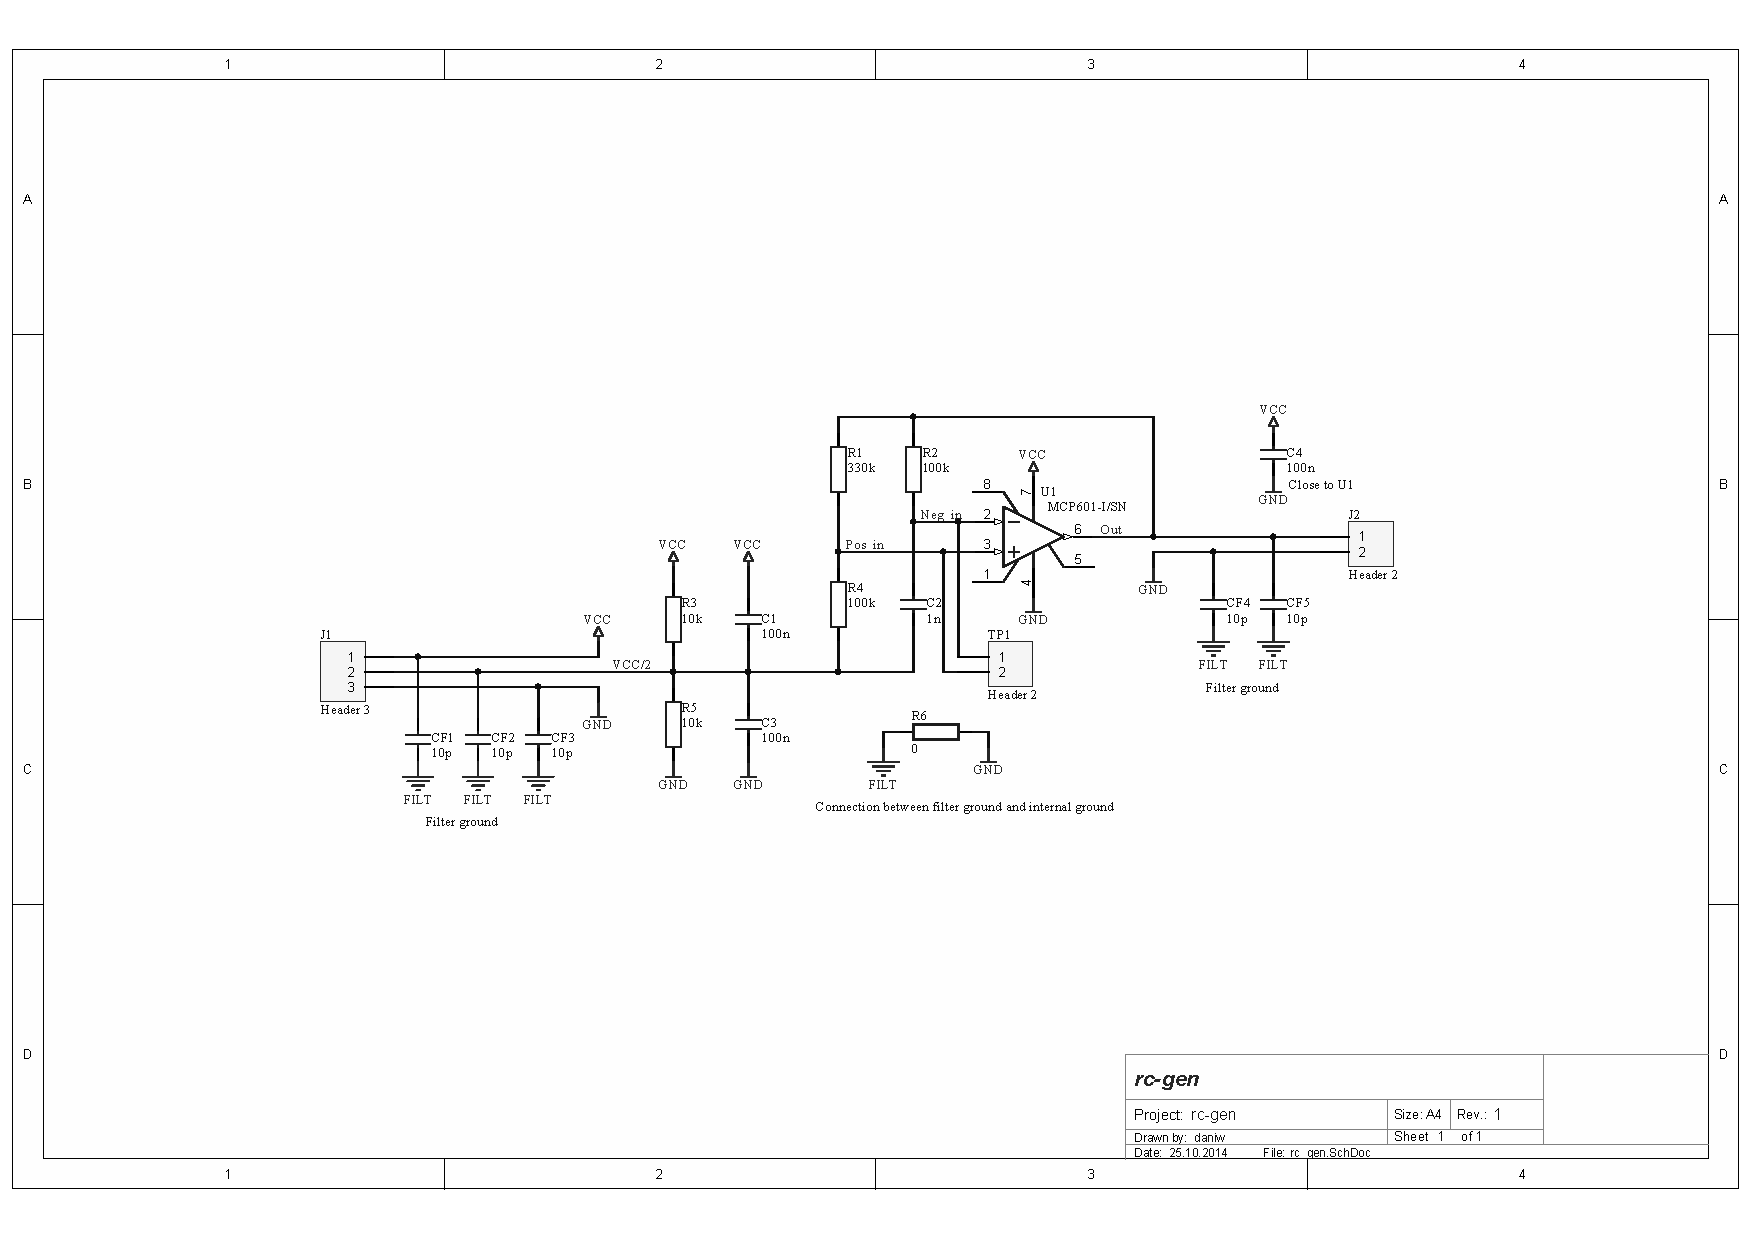
\includegraphics[width=\textwidth]{../rc-gen/rc-gen-sch.PDF}
    \caption{Schema rc-gen}
    \label{fig:schematic}
\end{figure}
\noindent
Die Schaltung beinhaltet einen RC Oszillator. Dieser besteht aus einem 
Operationsverstärker als Schmitt Trigger beschaltet und einer Mitkopplung. 
Da die Schaltung Single Supply gespiesen wird, generieren R3, R5, C1 und C3 
einen virtuellen Nullpunkt mit der halben Speisespannung. Die Hysterese wird 
mit R1 und R4 eingestellt. Die Schwingfrequenz wird mit R2 und C2 festgelegt. 
C4 dient dazu, die Speisespannung des Operationsverstärkers zu stützen. 
Die Kondensatoren CF1 bis CF5 leiten hochfrequente Störungen, welche über 
die Anschlüsse in die Schaltung gelangen könnten, zur Filtermasse ab. 
Die Filtermasse ist mittels R6 mit der Masse der Schaltung verbunden. 
Um die Schaltung besser ausmessen zu können, werden die Eingänge des 
Operationsverstärkers auf einen Anschluss geführt. 

\clearpage
\section{Layout}
\begin{figure}[h!]
    \centering
    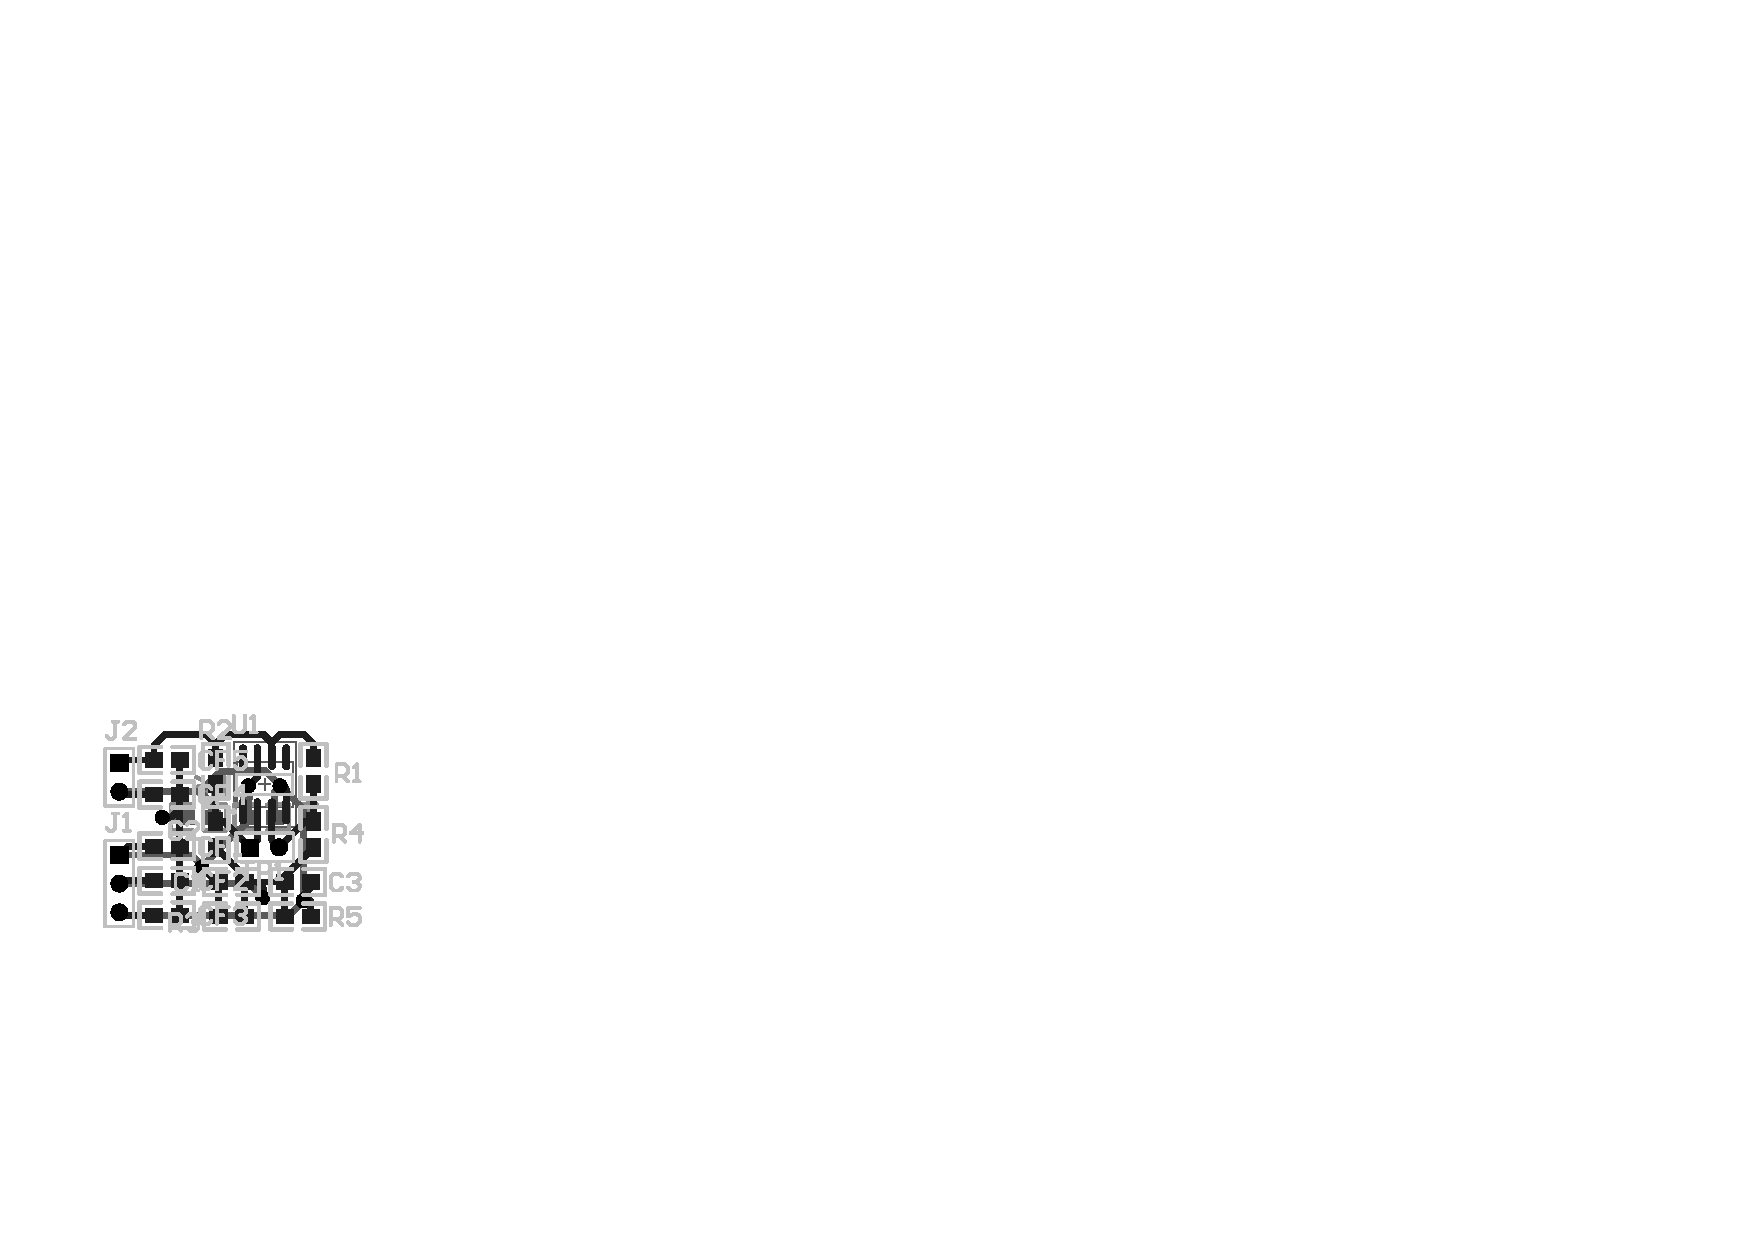
\includegraphics[width=0.8\textwidth]{../rc-gen/rc-gen-pcb.PDF}
    \caption{Layout rc-gen}
    \label{fig:layout}
\end{figure}
\noindent
Die Anschlüsse werden nahe aneinander platziert, um leitungsgebundene 
Störungen möglichst lokal zu halten. Die Entstörkondensatoren CF1 bis CF5 
werden nahe den entsprechenden Anschlüssen platziert und an die 
Filtermassefläche angeschlossen. Die Schaltung ist sehr kompakt aufgebaut, um 
mögliche Stromschleifen möglichst klein zu halten. Aufgrund der kompakten 
Platzierung der Bauteile ist es nicht möglich, eine Fläche für die 
Versorgungsspannung zu erstellen. Deshalb wird ein Stützkondensator direkt 
unter dem Operationsverstärker vorgesehen. Die Filtermasse wird an der 
Berührungslinie mit der Masse der Schaltung verbundden. Ansonsten besteht 
keine elektrische Verbindung zwischen den Masseflächen. 

\end{document}
